Zum Zeitpunkt der Veröffentlichung des von mir ausgewählten wissenschaftlichen Artikels wurden viele
unterschiedliche Methoden zur 3D Objekterkennung vorgestellt. Einzelne Deskriptoren konnten sich 
bisher nicht als überlegen herausstellen. Es hat sich etabliert, die jeweiligen Deskriptoren
geschickt zu kombinieren, um deren Stärken zu nutzen und somit eine weitaus bessere Ergebnisse bei der Objekterkennung zu erzielen.
Dementsprechend wird der in \cite{scherer2010histograms} vorgestellte 3DHOG mit hoch-dimensionalen Merkmal-Vektoren
verglichen und eine Kombination dieser beiden in einem Experiment versucht.
\newline
Hauptmotivation für der 3DHOG waren unter anderem bereits erfolgreiche Anpassungen von 2D-Bild-Analyse Methoden auf 3D Objekterkennung. Es wurde sich für die Anpassung des bereits erfolgreichen HOG aus \cite{dalal2005histograms} entschieden.


\subsection{Grundbegriffe}
Im folgenden werde ich ein paar wichtige Grundbegriffe für diese Ausarbeitung erläutern. 

\subsubsection{Globaler und partieller Ansatz}
Bei der 3D Objekterkennung gibt es zwei verschiedene Ansätze. Der globale Ansatz, zu dem der 3DHOG gehört, betrachtet jeweils die komplette Form des 3D Models und es wird nach Ähnlichkeiten gesucht, während der partielle Ansatz nach lokalen Ähnlichkeiten sucht. Als ähnlich werden 2 Objekte betrachten, wenn deren Merkmale einen Schwellenwert bezüglich ihrer Differenz bzw. Distanz unterschreiten. Ähnlichkeit ist in der 3D Objekterkennung problematisch, da zusätzlich zu gegebenenfalls sich unterscheidender Beleuchtung noch der Betrachtungswinkel eine Rolle spielt. Bisher konnte diese Problematik noch nicht absolut gelöst werden, weder für den globalen noch für den partiellen Ansatz. Dementsprechend haben entsprechende Lösungsversuche einen heuristische Natur \cite{scherer2010histograms}.

\subsubsection{Histogramm}
Histogramme dienen in der Statistik und Bildverarbeitung dazu, Häufigkeiten bestimmter Merkmale visuell darzustellen. Ein einfaches Beispiel aus der Bildverarbeitung wäre ein Histogramm eines
Graustufenbildes mit den jeweils darin vorkommenden Grauwerten. Ein Beispiel für eine grafische Darstellung ist bei \figurename~\ref{histo_pic} zu finden.

\begin{figure}[thpb]
	\centering
	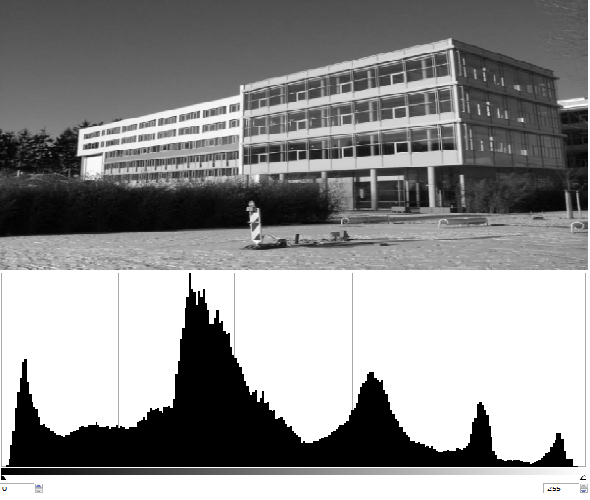
\includegraphics[width=\linewidth]{1-Einleitung/pics/pic_histo_uni01.png}
	\caption{Grauwertbild (entnommen aus Übungsmaterialien Bildverarbeitung 1 WS2015/2016) mit Histogramm (Erstellt mit GIMP 2.8.16)}
	\label{histo_pic}
\end{figure}


%\begin{table}[H]
%	\centering
%	\caption{Grauwert Histogramm}
%	\label{bsp Histogramm}
%	\begin{tabular}{ll}
%		Grauwert & Anzahl \\
%		150      & 30     \\
%		20       & 5      \\
%		...      & ...    \\
%		255      & 10    
%	\end{tabular}
%\end{table}

Eine detailreichere Einführung im Bezug auf Bildverarbeitung ist in \cite{Priese15} zu finden.

\subsubsection{Gerichtete Gradienten}
Gerichtete Gradienten werden wie z.B. in \cite{dalal2005histograms} äußerst erfolgreich zur Merkmaildetektion für 2D Bilder eingesetzt. Die Verwendung dieses Begriffs kann in \cite{scherer2010histograms} und dementsprechend in dieser Ausarbeitung vom mathematischen Begriff abweichen.
\newline
Um gerichtete Gradienten zu berechnen, benötigt man Gradientenoperatoren. Hiermit sind Lineare Filter aus der Bildverarbeitung gemeint. In der Einführungslektüre \cite{Priese15} versteht man Filter als Funktionen, welche auf Bilder, als Matrizen darstellbar, angewendet werden. Gradientenoperatoren sind gemäß der Definition über differenzierbare Funktionen, eine entsprechende Approximation mit denen man z.B. 2D Bilder "`ableiten"' kann. Die Filtermaske \ref{Abl_Maske} 

\begin{equation}
\label{Abl_Maske}
\begin{bmatrix}
-1 & 0 & 1
\end{bmatrix}
\end{equation}

bewirkt z.B. die 1. Ableitung. Dieser Filter kann z.B. für ein 2D Bild in die X-Richtung (Betrachtung der benachbarten Pixel links und rechts vom abzuleitenden Pixel) und in die Y-Richtung (Betrachtung der benachbarten Pixel über und unter dem Abzuleitenden Pixel) angewendet werden.  

\begin{table}[]
	\centering
	\caption{Grauwertbild als Matrix}
	\label{GrauwertMat}
	\begin{tabular}{llll}
		$a_{00}$ & $a_{01}$ & $a_{02}$ & $a_{03}$ \\
		$a_{10}$ & 100    & 50     & 235     \\
		$a_{20}$ & 73     & 42     & 150      \\
		$a_{30}$ & 30     & 125    & 0                     
	\end{tabular}
\end{table}

Formel \ref{abl_a22} zeigt ein Beispiel, wie ein Element aus \tablename~\ref{GrauwertMat} abgeleitet wird. In diesem Fall in X-Richtung. An den Rändern muss jeweils eine Randbehandlung vorgenommen werden. Werte können z.B. gespiegelt werden.
\begin{equation}
\label{abl_a22}
a_{22}'x = -73 + 0 +150 = 77
\end{equation}

Mit den Gradientenoperatoren lässt sich jeweils die Gradientenlänge bzw. -betrag und die Gradientenrichtung berechen. Die Formeln (\ref{Grad_L}) und (\ref{Grad_R}), entnommen aus \cite{Priese15} zeigen jeweils die Berechnung für 2D Bilder. $G_l$ ist der Gradientenbetrag und $G_r$ die Gradientenrichtung $I_x$ bzw. $I_y$ steht jeweils für die Ableitung in X- bzw. Y-Richtung. Mit dem Parameter p ist den entsprechende Pixel gemeint.
\begin{equation}
\label{Grad_L}
G_l(p) = \sqrt{I^2_x(p)+ I^2 y(p)}
\end{equation}

\begin{equation}
\label{Grad_R}
G_r(p) = arctan_2(- I_y(p),I_x(p))
\end{equation}


\subsubsection{3D Mesh}
3D Meshes werden dazu verwendet um 3D Objekte digital zu speichern. Es werden Informationen über die Vertices (Punkte), Kanten, Flächen, Polygone sowie falls nötig Informationen über die Oberfläche (z.B. Farbe) gespeichert. In dem ausgewählten Artikel \cite{scherer2010histograms} werden Meshes aus schon bestehenden Performanz-Tests genommen um die Leistungsfähigkeit des 3DHOG zu messen.